%!TEX root = ../dokumentation.tex

\chapter{Markt}

\section{Definition}

Die Bezeichnung was ein Smartphone genau ist, trifft diese Definition aus dem Wirtschaftslexikon Gabler gut:

\textit{Mobiltelefon mit erweitertem Funktionsumfang. Dazu zählen neben der Telefonie und Short Message Service (SMS) üblicherweise Zusatzdienste wie Electronic Mail (E-Mail), World Wide Web (WWW), Terminkalender, Navigation sowie Aufnahme und Wiedergabe audiovisueller Inhalte. Auf Smartphones laufen gegenüber herkömmlichen Mobiltelefonen komplexere Betriebssysteme wie etwa Symbian OS, Blackberry OS oder das iPhone OS. Die hierdurch geschaffene Möglichkeit zur Installation weiterer Applikationen durch den Endnutzer verleiht Smartphones einen erweiterbaren und individualisierbaren Funktionsumfang.}

Nachdem nun der Begriff abgegrenzt ist, werden wir im Folgenden auf die Geschichte und Entwicklung des Markts eingegangen.


\section{Geschichte und Entwicklung}

Laut dieser Definition gibt es das eigentliche Smartphone schon deutlich länger als viele Leute vermuten. Bereits 1994 entwickelte IBM ein damals „Personal Communicator “ genanntes tragbares Gerät. Weiter Anbieter kam auf den Markt dazu, sodass Anfang des 21. Jahrhunderts Windows Mobile, Blackberry OS und Palm OS zu den bekanntesten Systemen zählten. Allerdings waren diese Geräte nur wenigen Teilen der Bevölkerung vorenthalten  und wurden hauptsächlich im beruflichen Umfeld genutzt. Einen regelrechten Boom hat der Smartphonemarkt durch die Einführung des iPhone’s im Jahr 2007 erfahren. Von diesem Zeitpunkt an kamen weitere Anbieter hinzu, unteranderem Samsung und HTC. Diese Hersteller setzen davor zwar auch schon auf vorhandene Systeme, doch Apple verstand es am besten die Technik und Vorteile an den normalen Benutzer zu bringen und dies mit einer Einfachheit, dass auch Menschen mit wenig technischem Verständnis die Geräte bedienen konnten. Von diesen Ideen geprägt veränderten auch die anderen Hersteller ihr Produktportfolio und ihre Smartphones. Mit diesen Veränderungen wurde auf einmal ein viel größerer Markt möglich. Angefangen im Jahre 2007 mit 122 Millionen verkauften Einheiten, hat sich der Markt rasant entwickelt. In folgender Statistik sieht man, wie viel Potenzial noch in dem Markt steckt: 

\section{Aktuelle Situation}

Der Smartphonemarkt ist ein besonderer Markt. Anders als bei den Computern, wo Windows mit fast 90 Prozent stark dominiert, mischen auf dem Smartphonemarkt verschiedene Betriebssysteme mit. Auf die drei größten wird kurz eingegangen:

\textbf{Android}: wird von  der Open Handset Alliance entwickelt, deren Gründer Google ist. Auf Grund keiner Gebühren findet man es  auf sehr vielen Geräten wieder. Android basiert auf dem Linuxkernel und soll ein freies Betriebssystem sein. Die Hersteller der Handys können es nach Belieben modifizieren und eigene Oberflächen für die Nutzer bereitstellen.

\textbf{iOS}: ist das Betriebsystem von Apple. Im Gegensatz zu Android läuft es nur auf den Geräten von Apple, dazu zählt das iPhone , iPad und iTV. Es ist keine Modifikation des Betriebssystems möglich und Applikationen können ausschließlich über den eigenen Appstore installiert werden.
 
\textbf{WindowsPhone}:   ist das ehemalige WindowsMobile und der Versuch von Microsoft auch auf Smartphonemarkt mitzuspielen. Es wurde erst 2010 vorgestellt und ist damit im Vergleich zu den anderen Systemen das jüngste. Die Hersteller können entgegen einer Lizenzgebühr das Betriebssystem auf ihren Geräten installieren.


Im letzten Quartal 2013 wurden folgende Prozentsätze von den verschiedenen Systemen in Deutschland abgesetzt. An der Spitze steht Android mit fast 75 Prozent, gefolgt von iOS mit ca. 17 Prozent und dahinter WindowsPhone mit ca. 6 Prozent.
Viele Käufer nehmen eines der oben genannten Betriebssysteme als  eine Grundvoraussetzung für ihre Kaufentscheidung an. Weitere wichtige Entscheidungen werden in der folgenden, etwas älteren,  Statistik deutlich:


Ein entscheidender Punkt für den Kauf eines Gerätes stellen technische Features da. Auf Platz eins steht in dieser Umfrage die Akkulaufzeit, d.h. wenn ein Hersteller in diesen Bereich stark investiert und eine wichtige Entdeckung machen würde, hätte er einen guten Grund für den Verkauf des Gerätes. Ähnlich verhält es sich mit einer Vielzahl von anderen Punkten auf der Statistik, wie die hochwertige Kamera, ein großes Display oder der Touchscreen. Aus dieser Darstellung lässt sich erkennen dass die Forschung in dem Smartphonemarkt eine sehr wichtige Rolle spielt. Ohne einen Touchscreen würde sich heute eine Vielzahl an Modellen überhaupt nicht mehr verkaufen. Ein gutes Beispiel hierfür ist der Hersteller Blackberry. Früher einer der Vorreiter  im Enterprisebereich, heute hat er  sehr geringe Absatzzahlen und eine wirtschaftlich schwierige Lage. Einer der Gründe für die Situation war sicherlich, dass Blackberry zu lange an seinen klassischen Tastaturtelefonen festgehalten hat und nicht dem Trend nach neuen Entwicklungen gefolgt ist. Neben der Technik  spielt allerdings für 40 Prozent der Befragten allerdings auch ein bekannter Hersteller eine wichtige Rolle, dieser Punkt wird in der folgenden Käufergruppenanalyse nochmal genauer dargestellt.

Auch im Smartphonemarkt gibt es unterschiedliche Preissegmente und somit auch Käufergruppen. Zu dem hochpreisigen Sortiment zählen die iPhones und Top-Modelle von Samsung, Sony, Nokia  und HTC. Diese Modelle kosten bei ihrer Markteinführung meist über 500 Euro und deren Preis steigt meist noch weiter mit zusätzlichen internen Speicher. Typisch für die Modelle dieser Preisklasse sind technische Neuheiten, wie eine sehr hohe Displayauflösung oder eine besondere Kameratechnik. Die Nutzer sind bereit viel Geld auszugeben um auf dem neusten Stand der Technik zu sein. Außerdem finden sich in diesem Bereich zusätzlich Markenkäufer, d.h. Konsumenten die einem Hersteller treu bleiben. Typisch ist Markentreue für die Applegerätenutzern. 

Nach diesem hochpreisigen Bereich, gibt es auch ein mittelpreisiges Segment. Die Modelle kosten zwischen 200  und 500 Euro und  sind damit für eine größere Masse erschwinglich. Durch den niedrigeren Preis ist allerdings auch weniger Technik verbaut. Im Allgemeinen sind die Prozessoren nicht mehr so leistungsstark, das Display oder dessen Auflösung kleiner und keine absoluten neuen Features in das Gerät integriert. Die Nutzer dieser Smartphones, entsprechen dem Durchschnitt und wollen einige technische Möglichkeiten, jedoch nicht alle haben. Man könnte sie als Preis-Leistungs-Käufer bezeichnen.

Die letzte Käuferschicht, entspricht dem Bbllig Segment. Die Smartphones kosten unter 200 Euro und gehen im Preis herunter  bis zu hohen zweistelligen Beträgen. Die Hersteller, die hier ihre Produkte verkaufen, wollen vor allen Dingen einen hohen Marktanteil in der Bevölkerung erreichen und auch weniger technisch versierte Menschen damit ansprechen, sich ein Smartphone zu kaufen. Von den Features werden wenig eingebaut um den Preis maximal zu drücken zu können. Meist besitzen die Geräte eine schlechtere Kameras  und kleinere Displays.
Die oben beschriebenen drei Segmente schwanken natürlich, es gibt keine feste Abgrenzungsmöglichkeit. Es existieren auch Geräte die wenig Kosten und trotzdem gut ausgestattet sind.



\subsection{Besonderheiten}
Der letzte wichtige Punkt in dem Smartphonemarkt sind Patentstreitigkeiten. Patente sind gewerbliche Schutzrechte, die eine Firma auf technische Neuheiten anmelden kann. Da sich auf dem Smartphonemarkt in den letzten Jahren sehr viel entwickelt hat, wurde auch eine große Anzahl von Patenten angemeldet. Das hat zum Ziel das wichtige Entdeckungen nur in den eigenen Produkten zu finden sind und so einen Wettbewerbsvorteil vor dem Konkurrenten entsteht oder das Unternehmen zumindest Lizenzgebühren für die Verwendung ihrer Erfindung einnehmen kann.  Durch den hohen Druck auf dem Markt, verwenden viele Firmen jedoch einfach Technologien von Konkurrenten für die sie keine Genehmigung besitzen. Einer der größten Fälle, war die Klage von Apple gegen Samsung. Die zeitweise sogar ein Verkaufsverbot für ein Tablet von Samsung zur Folge hatte. Apple forderte ursprünglich eine Milliarde Dollar Schadensersatz von Samsung(http://www.heise.de/mac-and-i/meldung/Samsung-muss-Apple-weitere-290-Millionen-Dollar-Schadensersatz-zahlen-2052251.html)

Im Folgenden wird nun vereinfacht der Ablauf eines solchen Patentstreites dargestellt: Falls der Verdacht einer Verletzung der eigenen Patente vorliegt,  hat das patentbesitzende  Unternehmen grundsätzlich folgende Rechte:
\begin{itemize}
\item  Unterlassung des Verkaufs des geschützten Gegenstandes
\item  Zahlung von Schadensersatz
\item  Produkte des Konkurrenten aus dem Markt entfernen
\item  Erhalt genauer Zahlen über den Verkauf der geschützten Erzeugnisse
\end{itemize}

Der Schadensersatz kann aus drei möglichen Faktoren berechnet werden. Zum ersten dem entgangenen Gewinn des patentbesitzenden Unternehmens, zum zweiten die Herausgabe des Gewinns die das gegnerische Unternehmen durch die Verletzung der Patente erzeugt hat und dritten die Zahlung von Lizenzgebühren. Verhärtet sich der Verdacht, dass der Konkurrent keine Rechte an der eingesetzten Technologie hat, kann das patentbesitzende Unternehmen versuchen die oben genannten Rechte durchzusetzen. Im allgemeinen Fall wird zu erste eine Abmahnung verschickt mit einer geforderten  Schadenssumme. Selten jedoch geht das gegnerische Unternehmen im Smartphonemarkt darauf ein, da es sich meist um große Konzerne handelt. Um sich nun auf die Klage vorzubereiten ist eine sorgfältige Planung und Analyse des Sachverhaltes nötig, denn das klagende Unternehmen trägt die Beweislast. D.h. das Gericht stellt keine Nachforschungen an sondern bewertet nur die ihm vorgelegten Erkenntnisse. Oft dauert der Prozess über mehre Verhandlungstage hin bis zu Jahren wie in dem Fall  Apple vs. Samsung,  der schon seit April 2011 läuft. Entweder verhängt das Gericht dann ein Verkaufsverbot oder fordert eine Schadensersatzzahlung von dem verurteilten Unternehmen.

Da diese Patentstreitigkeiten sich, wie beschrieben, oft länger hinziehen können, muss ein Unternehmen auch genug Geld haben um seine eigene Rechtsabteilung mit den Anwälten zu bezahlen. Verliert das Unternehmen den Rechtsstreit muss es in Normalfall auch die Gerichtskosten des Gewinners tragen, zusätzlich zu dem Schadensersatz oder andere Ansprüche, die es sowieso bezahlen muss. Ein Gerichtsverfahren kann sehr teuer werden. Aus diesem Grund heraus haben viele Smartphonehersteller Patente und Lizenzen von anderen Unternehmen erworben um gegen solche Streitigkeiten gewappnet zu sein.

\section{Spielprinzip}
Das im Folgenden dargestellte Spiel „Avalon“ soll rundenbasiert verlaufen sein. Darunter versteht man, dass nach jeder abgeschlossenen Runde die Simulation startet und für die nächste Runde neue Ausgangsbedingungen schafft. Jeder Spieler legt also in der aktuellen Runde seine Tätigkeiten für die nächste Periode fest und trifft Entscheidungen. Danach wir gewartet bis jeder Spieler seine Runde abgeschlossen hat, darauf folgt die Simulationsphase, die alle Tätigkeiten der Spieler erfasst und umsetzt. In der nächsten Runde beginnt das Ganze von vorne. Jeder Teilnehmer des Wirtschaftssimulationsspiels soll dabei von seinem eigenen Rechner aus spielen können und nicht wie bei dem „hot seat“ Verfahren, alle Mitspieler an einem Computer abwechselnd. Die Hauptaufgabe besteht darin die verschiedenen Abteilungen zu koordinieren. In dem Spiel werden die Produktion, der Verkauf, der Einkauf, das Marketing, die Forschung und die Rechtsabteilung abgebildet. Jede dieser Abteilungen hat fixe Kosten die immer anfallen und variable kosten, die nur anfallen wenn etwas in der Abteilung gemacht wird. Der Spieler soll die Möglichkeit bekommen, strategische Schwerpunkte zu setzen, in dem er einzelne Abteilungen z.B. stärker finanziert als andere. Außerdem soll durch Zufallsereignisse das Spiel spannend gehalten und eine Monotonie vermieden werden.

\subsection{Abteilungen}
In diesem Kapitel werden  die Abteilungen näher erläutert.

\textbf{Produktion: }
In dieser Abteilung kann das aktuelle Smartphone produziert werden. Die Herstellung älterer Modelle ist nicht möglich. Für die Produktion  werden Ressourcen benötigt und zwar pro Smartphone immer eine. Ein Upgrade dieser Abteilung hat geringere Ausschussquoten  und somit auch weniger unnötig gekaufte Ressourcen zur Folge, verursacht jedoch höhere Fixkosten. Für die Produktion eines Smartphones fallen variable Kosten an.

\textbf{Verkauf:} 
In der Verkaufsabteilung werden alle Produkte, die sich im Lager des Unternehmens befinden angezeigt. Ältere Modelle können solange verkauft werden, wie sie noch vorhanden sind, jedoch wie oben beschrieben nicht mehr produziert. Um ein Modell zum Verkauf auf dem Markt freizugeben, genügt es einen Preis für dieses festzulegen.

\textbf{Einkauf:} 
Im Einkauf steht die Ressourcenbeschaffung im Vordergrund. In diesem Spiel hat der Nutzer die Möglichkeit sich zwischen drei Lieferanten zu entscheiden. Jeder dieser Lieferanten hat unterschiedliche Preise, Qualität und Zuverlässigkeit. Eine erhöhte Qualität hat einen geringeren Ausschuss bei der Produktion zur Folge und die Zuverlässigkeit erhöht die Planbarkeit des Unternehmens, denn falls dieser Wert gering ist, wird eine Lieferverzögerung häufiger auftreten.

\textbf{Forschung:} 
Die Forschungsabteilung ist ein sehr wichtiger Bestandteil der Firma. Grundsätzlich kann der Spieler Forschungskampagnen für Display, Prozessor und Akku starten. Jede der Kampagnen hat drei festgelegte Werte neben ihren Preis, die Erfolgswahrscheinlichkeit, die Dauer und die mögliche Levelsteigerung. Die Erfolgswahrscheinlichkeit gibt an, mit welchem Prozentsatz  eine neue Entwicklung gemacht wird. In der Dauer ist festgelegt wie viel Zeit vergeht, bis die Resultate der Kampagne bekannt werden. Falls nun die Kampagne geglückt ist wird der Wert der Levelsteigerung auf das aktuelle Forschungslevel addiert. Um sich nun gegen kommende Klagen zu schützen, kann der Spieler sein aktuellen Level gegen einen gewissen Geldbetrag patentieren lassen. Die Erfolgswahrscheinlichkeit der Kampagnen steigt durch ein Upgrade der Abteilung an, dies hat jedoch höhere Fixkosten zur Folge. Falls der Spieler wenig Geld investieren will, gibt es zusätzlich noch die Möglichkeit einen Konkurrenten auszuspionieren. Durch eine erfolgreiche Spionage steigt das eigene Forschungslevel an. Allerdings kann die Spionage auch auffliegen und rechtliche Konsequenzen folgen. Von der Forschungsabteilung kann der Spieler nun ein neues Produkt in die Produktion geben und somit das alte ersetzen.

\textbf{Marketing: }
Ähnlich wie in der Forschungsabteilung kann der Spieler im Marketing auch Kampagnen starten. Es wird zwischen einer Printmedien-, einer Internet- und einer Fernsehkampagne unterschieden. Neben unterschiedlichen Kosten unterscheiden die sich Marketingmaßnahmen in der Laufzeit, dem Imageupgrade und der Erfolgswahrscheinlichkeit. Das Imageupgrade erhöht nachher die Absatzchancen auf dem Markt. Wie bei der Forschungsabteilung auch, kann die Erfolgswahrscheinlichkeit durch ein Upgrade, welches höhere Fixkosten verursacht, erhöht werden.

\textbf{Rechtsabteilung:} 
In der Rechtsabteilung kann der Spieler seine Konkurrenten auf Spionageaktivitäten bei ihm prüfen. Wird eine Spionagekampagne gefunden kann er den Gegenspieler verklagen. Ein Upgrade der Abteilung bringt höhere Siegchancen im Rechtsstreit mit sich.

\section{User Interface}
Dies war das erste Mockup der Benutzeroberfläche:

\begin{figure}
\centering
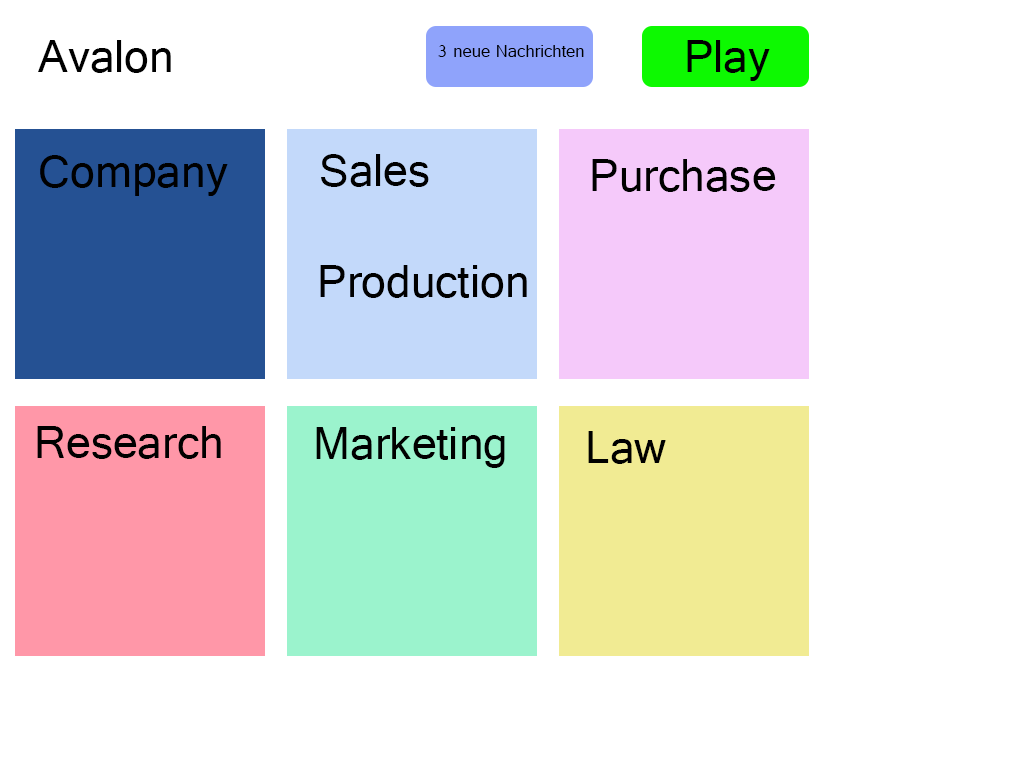
\includegraphics[width=0.7\linewidth]{../images/mockup1}
\caption{Mockup1}
\label{fig:mockup1}
\end{figure}


In der oberen Zeile, hat der Spieler die Möglichkeit seine Nachrichten zu lesen und durch das drücken des Playbuttons die Runde zu beenden. In diesem Entwurf wurde davon ausgegangen, das sich durch einen Klick auf die Panels ein Popup-Fenster öffnet in dem der Nutzer seine Eingaben und Entscheidungen für die jeweilige Abteilung festlegt.  Das zweite Mockup setzte jedoch schon auf eine andere Möglichkeit:

\begin{figure}
\centering
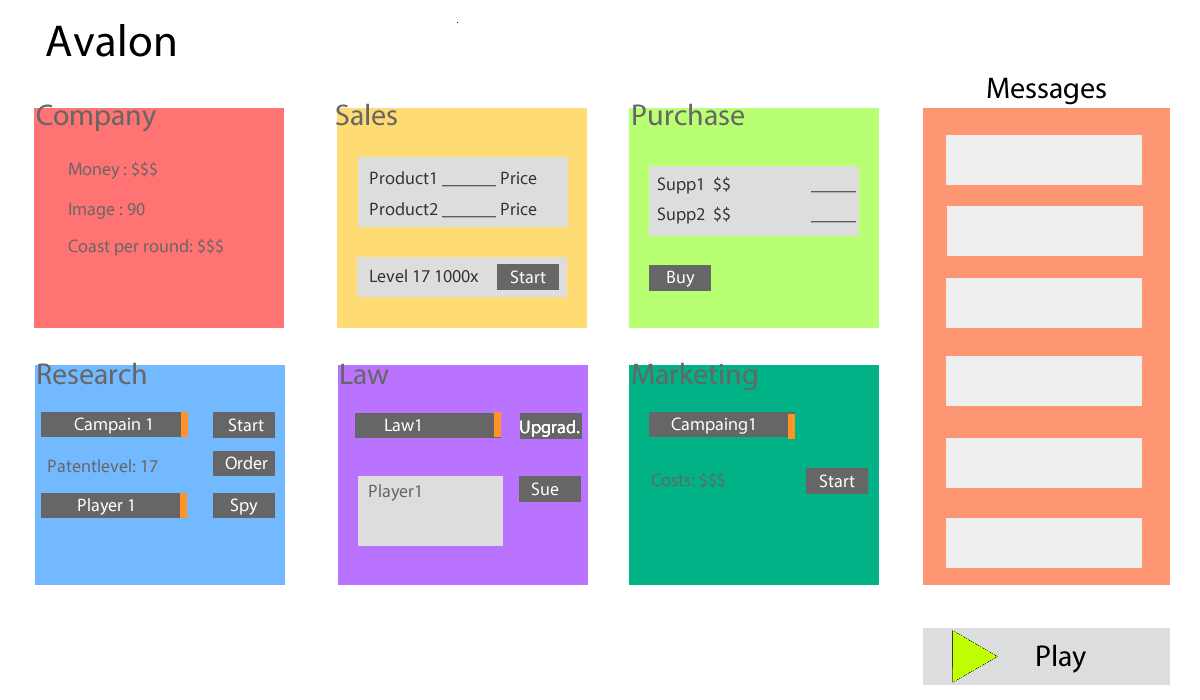
\includegraphics[width=0.7\linewidth]{../images/mockup2}
\caption{Mockup 2}
\label{fig:mockup2}
\end{figure}

Das neuen Mockup ist darauf ausgelegt worden, dass sich für die Bedienung des Spiels keine weiteren Fenster mehr öffnen müssen. Die einzige Ausnahme ist das Lesen einer Nachricht. Ansonsten kann der Spieler alle Einstellungen direkt vornehmen. In dem Companypanel werden grundsätzliche Informationen wie das Geld und die Fixkosten angezeigt, die restlichen Abteilungen funktionieren wie beschrieben.
Das Spiel sieht letztendlich so aus:

\begin{figure}
\centering
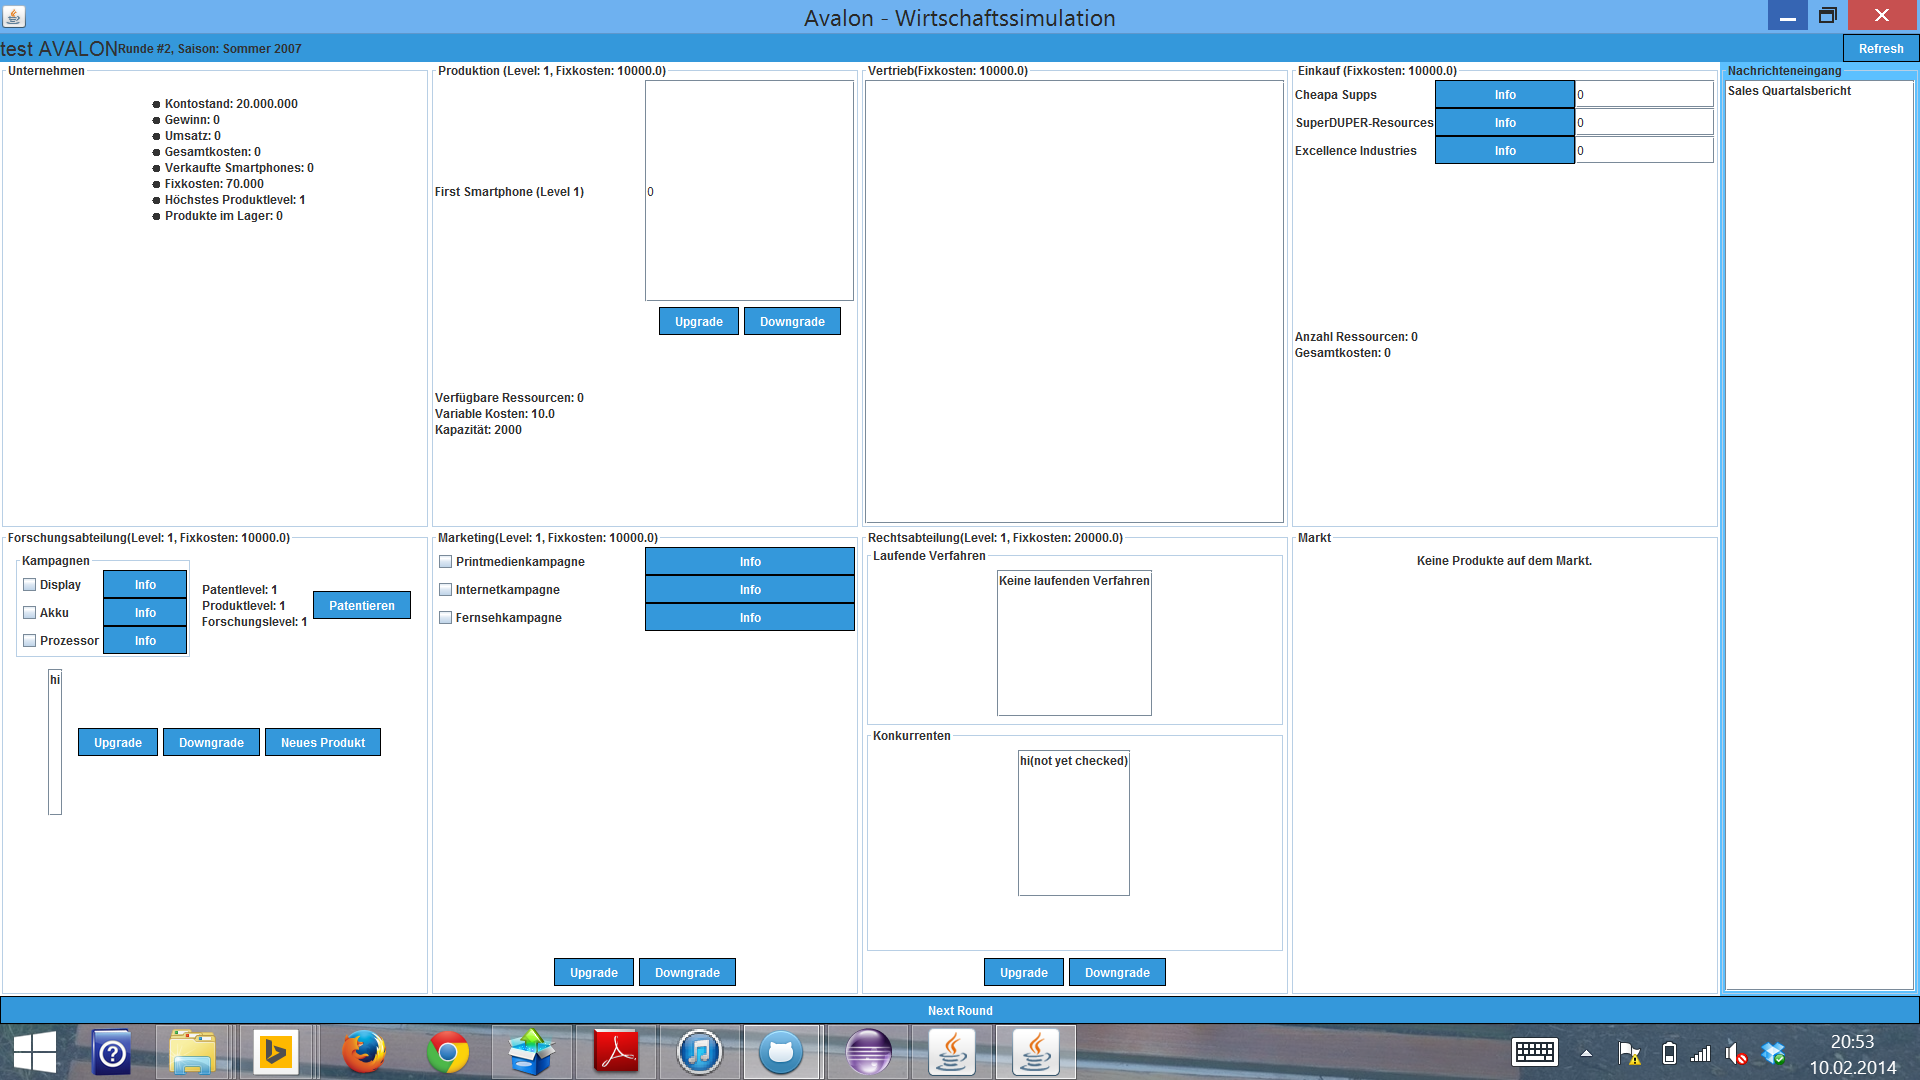
\includegraphics[width=0.7\linewidth]{../images/mockup3}
\caption{Screenshot}
\label{fig:mockup3}
\end{figure}









